\documentclass[paper=b5,fontsize=10pt]{jlreq}
\usepackage{
  amsmath,amssymb,mathtools,
  fontset-public,KKsymbols,luwa-ul,
  enumitem,fancyhdr,
  wrapfig2,luatexja-otf,modernruler,
  tikz
}
\usepackage[unit=1\zw,tensenoff=0pt]{KKran}
\usepackage[left=20mm,right=20mm,top=30mm,bottom=0mm]{geometry}
\usetikzlibrary{calc,intersections,angles,quotes}

\pagestyle{fancy}
\renewcommand{\headrule}{\relax}
\fancyhead{\relax}
\fancyfoot[C]{\symbol{"2015}\hspace*{.5\zw}\thepage\hspace*{.5\zw}\symbol{"2015}}

\newlist{densemondai}{enumerate}{1}
\setlist[densemondai,1]{
  label=\kakko{\arabic*},leftmargin=1\zw,
  listparindent=1\zw,labelsep=1\zw,itemindent=1\zw,
  topsep=0mm,itemsep=\baselineskip
}
\newlist{mondai}{enumerate}{2}
\setlist[mondai,1]{
  label=\kakko{\arabic*},leftmargin=1\zw,
  listparindent=1\zw,labelsep=1\zw,itemindent=1\zw,topsep=0mm
}
\setlist[mondai,2]{
  label=\kakko{\mruleth[height=.7\zw,width=0pt]\Rrnum{\arabic*}},
  leftmargin=1\zw,listparindent=1\zw,labelsep=1\zw,itemindent=1\zw,topsep=0mm
}

\NewDocumentCommand{\ExamTitle}{m}{%
  \begin{center}
    \LARGE\underLineKK[height=.8pt]{\makebox[5\zw][s]{第#1問}}
  \end{center}
  \vspace{\baselineskip}
}
\NewDocumentCommand{\ScratchPage}{}{%
  \newpage
  \begin{center}
    \underLineKK[height=.8pt]{\makebox[8\zw][s]{計算用紙}}
  \end{center}
}

\NewDocumentCommand{\年度}{}{20XX}
\NewDocumentCommand{\回数}{}{X}
\NewDocumentCommand{\日時と時刻}{}{20XX年X月X日\kakko{X}\hspace{1\zw}（100分）}

\begin{document}

\begin{titlepage}
  \begin{center}
    {\Huge
      \年度 年度\hspace{\zw}第\回数 回\\[.3\baselineskip]
      中2校内模試問題\\[.3\baselineskip]
      数学
    }\\[.3\baselineskip]
    {\Large
      （配点120点）\\[\baselineskip]
      \mbox{\日時と時刻}
    }\\[\baselineskip]
    {\Large\makebox[8\zw][s]{注意事項}}\\[\baselineskip]
    \begin{itemize}[itemsep=.3\baselineskip,labelsep=\zw,itemindent=\zw,leftmargin=0\zw]
      \item[1] 試験開始の合図があるまで、この問題冊子を開いてはならない。
      \item[2] 落丁、乱丁または印刷不鮮明の箇所を見つけた場合は、監督者に申し出よ。
      \item[3] すべての解答用紙の指定欄に、受験番号と氏名を記入せよ。
      \item[4] 解答は、必ず解答用紙の指定された箇所に記入せよ。
      \item[5] 答えだけを求める問題を除き、考え方や計算の過程も記すこと。
      \item[6] \namiKK{\HiraginoKakuGothic{3}本資料は鉄緑会公式のものではなく、作成・配布は同会と無関係な個人が行うものである。}
    \end{itemize}
    \vspace{\baselineskip}
    \KKran{\小問欄{5}{3}[center={受験番号}]\小問欄{7}{3}\小問欄{3}{3}[center={氏名}]\小問欄{20}{3}}%
    \\[.3\baselineskip]
    上欄に受験番号・氏名を記入せよ。\\[\baselineskip]
    {\Huge 鉄\ichimoji{マネ}会\hspace{\zw}数学科}
  \end{center}
\end{titlepage}

\newgeometry{left=18mm,right=18mm,top=20mm,bottom=20mm}

\ExamTitle{1}
次の各問に答えよ。\underLineKKAuto[height=.7pt]{\HiraginoKakuGothic{3}本問は答えのみを記せばよい。}

\vspace{\baselineskip}
\begin{densemondai}
  \item 方程式 $x^2-5x+4=0$ を解け。
  \item 方程式 $x^3-6x^2+11x-6=0$ を解け。
  \item 方程式 $x^4-10x^2+9=0$ を解け。
  \item 2次のモニックな整式 $A,B$ の最大公約数が $x-1$、最小公倍数が
        $x^3-2x^2-x+2$ であるとき、$A,B$ を求めよ。
  \item $\displaystyle\frac{x-1}{x+1}-\frac{x+1}{x+2}$ を計算せよ。
  \item 次の数の中から、有理数をすべて選べ。
  \[
    -\sqrt{16},\quad \sqrt{18},\quad 0.1\dot{2}\dot{7},\quad
    \frac{13}{37},\quad \sqrt{0.81},\quad \pi-3
  \]
  \item $\displaystyle\frac{1}{\sqrt2+\sqrt3}$ の分母を有理化せよ。
  \item $\sqrt{9+4\sqrt5}$ の二重根号を外せ。
\end{densemondai}

\ScratchPage

\newpage
\ExamTitle{2}
次の各問に答えよ。

\vspace{\baselineskip}
\begin{mondai}
  \item $a>2$ で、$\sqrt{x}=\dfrac{a-2}{2}$ のとき、
        $\sqrt{4x+8a}$ を $a$ を用いて表せ。
  \item 白球4個、赤球3個、青球2個が入った袋から同時に2個を取り出す。
        2個が異なる色である確率を求めよ。
  \item 1回300円で引くくじが20本あり、賞金は次の表のとおりである。
  \begin{center}
    \renewcommand{\arraystretch}{1.25}
    \begin{tabular}{c|c|c}
      \hline
      等級 & 本数 & 賞金 \\\hline
      1等 & 1本 & 3000円 \\
      2等 & 3本 & 800円 \\
      3等 & 6本 & 200円 \\
      はずれ & 10本 & 0円 \\\hline
    \end{tabular}
  \end{center}
  賞金の期待値を求め、期待値の観点からこのくじを引くべきか判定せよ。
  \item $x+y+z=0$ のとき、$x^3+y^3+z^3-3xyz$ の値を求めよ。
  \item 4種類の菓子が十分な個数ある。合計10個を選び、どの種類も少なくとも
        1個は選ぶ方法は何通りあるか。
\end{mondai}

\ScratchPage

\newpage
\ExamTitle{3}
次の命題について、真ならば証明し、偽ならば反例を1つ挙げよ。
ただし、$\sqrt2,\sqrt3$ が無理数であることは証明なしで用いてよい。

\vspace{\baselineskip}
\begin{mondai}
  \item $\sqrt2+\sqrt3$ は無理数である。
  \vspace{1.2\baselineskip}
  \item 無理数 $\alpha$ に対して、$\alpha^2$ は無理数である。
  \vspace{1.2\baselineskip}
  \item 有理数 $x,y$ に対して、$x+y\sqrt2=0$ ならば $x=y=0$ である。
  \vspace{1.2\baselineskip}
  \item 実数 $x,y$ に対して、$x^2+y^2=0$ ならば $x=y=0$ である。
\end{mondai}

\ScratchPage

\newpage
\ExamTitle{4}
係数を前から読んでも後ろから読んでも同じになる方程式を相反方程式という。
以下の問いに答えよ。ただし、必要ならば $t=x+\dfrac1x$ とおいてよい。

\vspace{\baselineskip}
\begin{mondai}
  \item $\displaystyle x+\frac1x=4$ のとき、$x$ の値を求めよ。
  \item $x>0$ かつ $\displaystyle x^2+\frac1{x^2}=7$ のとき、次を求めよ。
  \begin{mondai}
    \item $\displaystyle x+\frac1x$
    \item $\displaystyle x^3+\frac1{x^3}$
    \item $\displaystyle x^4+\frac1{x^4}$
  \end{mondai}
  \item 方程式 $x^4-2x^3-x^2-2x+1=0$ を解け。
  \item 方程式 $x^5+2x^4-3x^3-3x^2+2x+1=0$ を解け。
\end{mondai}

\ScratchPage

\newpage
\ExamTitle{5}
鋭角三角形 $\mathrm{ABC}$ の外心を $\mathrm O$、重心を $\mathrm G$、垂心を $\mathrm H$ とする。
原点を $\mathrm O$ とし、点 $\mathrm A,\mathrm B,\mathrm C$ の位置ベクトルをそれぞれ
$\boldsymbol a,\boldsymbol b,\boldsymbol c$ とする。

\begin{center}
\begin{tikzpicture}[scale=.82,line cap=round,line join=round]
  \coordinate (A) at (.8,4.5);
  \coordinate (B) at (-3,0);
  \coordinate (C) at (4,0);
  \coordinate (O) at (.5,.9);
  \coordinate (G) at (.6,1.5);
  \coordinate (H) at (.8,2.7);
  \draw (A)--(B)--(C)--cycle;
  \draw[gray] (O)--(H);
  \foreach \P/\pos in {A/above,B/below left,C/below right,O/below,G/left,H/right}
    {\fill (\P) circle (1.2pt) node[\pos,font=\scriptsize] {$\mathrm{\P}$};}
\end{tikzpicture}
\end{center}

次の問いに答え、3点 $\mathrm O,\mathrm G,\mathrm H$ が一直線上にあることを示せ。
\vspace{\baselineskip}
\begin{mondai}
  \item 点 $\mathrm H$ の位置ベクトルが
        $\boldsymbol a+\boldsymbol b+\boldsymbol c$ であることを示せ。
  \item 点 $\mathrm G$ の位置ベクトルを
        $\boldsymbol a,\boldsymbol b,\boldsymbol c$ で表せ。
  \item 3点 $\mathrm O,\mathrm G,\mathrm H$ が一直線上にあり、
        $\mathrm{OG}:\mathrm{GH}=1:2$ であることを示せ。
\end{mondai}

\newpage
\ExamTitle{6}
方眼上の点 $\mathrm O(0,0)$ から点 $\mathrm P(5,5)$ まで、右または上に1だけ進む最短経路を考える。
点 $\mathrm A(2,3)$、点 $\mathrm B(3,2)$ とし、次の各問に答えよ。

\vspace{\baselineskip}
\begin{mondai}
  \item 最短経路の総数
  \item 点 $\mathrm A$ を通る最短経路の数
  \item 点 $\mathrm A$ を通らない最短経路の数
  \item 点 $\mathrm A$ または点 $\mathrm B$ の少なくとも一方を通る最短経路の数
  \item 直線 $y=x$ より上側へ出ない最短経路の数
  \item 直線 $y=x$ と端点以外で交わらず、かつ同直線より上側へ出ない最短経路の数
\end{mondai}

\vspace{1.1\baselineskip}
\begin{center}
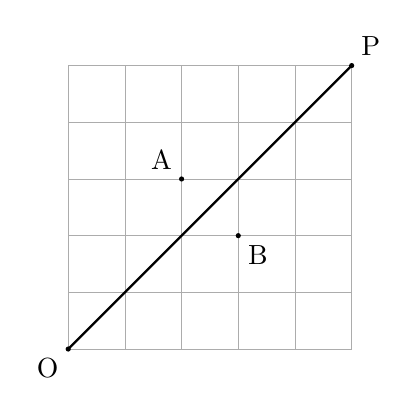
\begin{tikzpicture}[scale=.72]
  \draw[step=1,gray!65,very thin] (0,0) grid (5,5);
  \draw[thick] (0,0)--(5,5);
  \fill (0,0) circle (1.3pt) node[below left] {$\mathrm O$};
  \fill (5,5) circle (1.3pt) node[above right] {$\mathrm P$};
  \fill (2,3) circle (1.3pt) node[above left] {$\mathrm A$};
  \fill (3,2) circle (1.3pt) node[below right] {$\mathrm B$};
\end{tikzpicture}
\end{center}

\ScratchPage

\end{document}

